% `template.tex', a bare-bones example employing the AIAA class.
%
% For a more advanced example that makes use of several third-party
% LaTeX packages, see `advanced_example.tex', but please read the
% Known Problems section of the users manual first.
%
% Typical processing for PostScript (PS) output:
%
%  latex template
%  latex template   (repeat as needed to resolve references)
%
%  xdvi template    (onscreen draft display)
%  dvips template   (postscript)
%  gv template.ps   (onscreen display)
%  lpr template.ps  (hardcopy)
%
% With the above, only Encapsulated PostScript (EPS) images can be used.
%
% Typical processing for Portable Document Format (PDF) output:
%
%  pdflatex template
%  pdflatex template      (repeat as needed to resolve references)
%
%  acroread template.pdf  (onscreen display)
%
% If you have EPS figures, you will need to use the epstopdf script
% to convert them to PDF because PDF is a limmited subset of EPS.
% pdflatex accepts a variety of other image formats such as JPG, TIF,
% PNG, and so forth -- check the documentation for your version.
%
% If you do *not* specify suffixes when using the graphicx package's
% \includegraphics command, latex and pdflatex will automatically select
% the appropriate figure format from those available.  This allows you
% to produce PS and PDF output from the same LaTeX source file.
%
% To generate a large format (e.g., 11"x17") PostScript copy for editing
% purposes, use
%
%  dvips -x 1467 -O -0.65in,0.85in -t tabloid template
%
% For further details and support, read the Users Manual, aiaa.pdf.


% Try to reduce the number of latex support calls from people who
% don't read the included documentation.
%
\typeout{}\typeout{If latex fails to find aiaa-tc, read the README file!}
%


\documentclass[]{aiaa-tc}% insert '[draft]' option to show overfull boxes

 \title{Uncertainty Quantification Pertinent to Wind Farm Flow Physics and Modeling}

 \author{
    Pankaj K. Jha%
    \thanks{Senior Researcher, Wind Center of Excellence, AIAA Member.},\
    Kyle S. Hutchings%
   \thanksibid{1},\ and 
    Gregory S. Oxley%
   \thanks{Senior Manager, R \& D, Wind Center of Excellence, AIAA Member.}\\
  {\normalsize\itshape
   Envision Energy USA Ltd., Houston, TX 77002, USA}\\
  \and
  Sven Schmitz %
   \thanks{Associate Professor, Department of Aerospace Engineering, Senior AIAA Member.}\\
  {\normalsize\itshape
  The Pennsylvania State University, University Park, PA 16802, USA}
 }

 % Data used by 'handcarry' option if invoked
 \AIAApapernumber{YEAR-NUMBER}
 \AIAAconference{Conference Name, Date, and Location}
 \AIAAcopyright{\AIAAcopyrightD{YEAR}}

 % Define commands to assure consistent treatment throughout document
 \newcommand{\eqnref}[1]{(\ref{#1})}
 \newcommand{\class}[1]{\texttt{#1}}
 \newcommand{\package}[1]{\texttt{#1}}
 \newcommand{\file}[1]{\texttt{#1}}
 \newcommand{\BibTeX}{\textsc{Bib}\TeX}

\begin{document}

\maketitle

\begin{abstract}
This paper attempts to identify and quantify the uncertaintities associated with the modeling of wind farm and flow physics in wind farms. Different aspects and types of uncertainties in modeling the atmosphere are explained. This is followed by a description of the uncertainties in rotor modeling using different methods such as actuator disk method, generalized actuator disk, and actuator line method. This is further exemplified using the aleatoric and epistemic uncertainties in blade loads as a result of using actuator line method, followed by a discussion on the propagation of these uncertainties downstream. A formal stochastic analysis of the wind farm flow-field is ongoing and will be presented in the full paper.    
\end{abstract}

\section*{Nomenclature}

\begin{tabbing}
  XXXXX \= \kill% this line sets tab stop
  $ADM$ \> Actuator disk method \\
  $ABL$ \> Atmospheric boundary layer \\
  $AEP$ \> Annual energy production \\
  $ALM$ \> Actuator line method \\
  $COE$ \> Cost-of-energy \\
  $GAD$ \> Generalized actuator disk \\
  $LES$ \> Large-eddy simulation \\
  $NBL$ \> Neutral boundary layer \\
  $NREL$ \> National Renewable Energy Laboratory \\
  $SSC$ \> Stochastic simplex collocation \\
  $TKE$ \> Turbulent kinetic energy \\
  $UQ$ \> Uncertainty quantification \\
  $$ \>
 \end{tabbing}

\section{Introduction}

A true physical understanding of the subtleties involved in the operation of a wind farm is an open research problem. Wind farms operate under a range of atmospheric conditions and over a range of terrain. The goal of wind farm operators is to have the best possible assessment of wind resources for farm siting, blade loads, and blade fatigue to understand the structural health and life span of wind turbines. A very good understanding of wakes in a wind farm is necessary to assess the array efficiency, capacity factor, and Annual Energy Production (AEP). Several state-of-the-art models for atmosphere, wind turbines, and the wakes exist. These models vary significantly in complexity and fidelity. It is very important to identify the most critical aspects of the modeling chain by quantifying the associated uncertainties such as atmospheric stability, boundary conditions, turbulence model, turbine modeling approach, etc. This is necessary to define the range of applicability of these models and to develop best practices guidelines under these uncertainties. These, in turn, will provide the farm operators the knowhow to optimize the AEP. This abstract gives a description of the research problem and numerical methods, followed by an example and some planned techniques to be used. The proposed work will build on the latest advances in industry as well as in academia, including those by the authors. Different types of uncertainties associated with atmosphere and wind farm modeling will be identified. These uncertainties will be quantified with applications to wind farm simulations of different complexity. The enhanced understanding of wind farms operating under these uncertainties will help in better and effcient planning and operation of wind farms.

\section{Problem Description}
Though being one of the fastest growing sources of renewable energy, wind energy research faces a number of challenges today. One of the many difficulties involves an incomplete understanding of the turbine models and turbulence transport phenomena in a wind farm. This includes the understanding of atmospheric stability state, terrain, turbine modeling approaches, blade loads, fatigue, blade-loads-wake correlation, wake-wake and wake-atmospheric turbulence interaction.  Figure~\ref{f:HornsRev} shows the wake in Horns Rev wind farm. An idea of the complexity of the problem can be gained from figure~\ref{f:HornsRev}.

\begin{figure}
 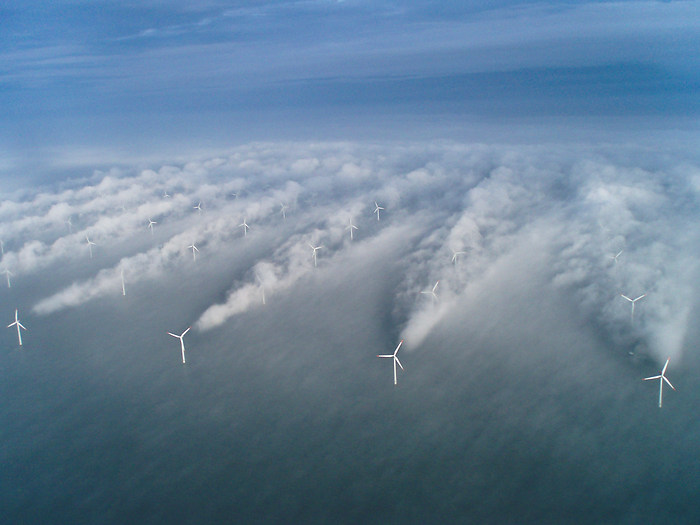
\includegraphics[scale=0.5]{HornsRev.png}
 \caption{Horns Rev Wind Farm.}
 \label{f:HornsRev}
\end{figure}

The associated array performance has a strong correlation with the spatial distance between turbines in an array. A well-designed utility-scale wind turbine can extract up to 50 percent of the wind power passing through its rotor disk area. The resulting viscous shear layer requires some distance to develop and to restore the momentum and energy that have been extracted by an upstream wind turbine. Moreover, the meandering of wakes from wind turbines from an adjacent row can cause span-wise shear in velocity and further complicate the flow field in front of a downstream turbine. Therefore, in the wind energy community, the accurate computation of the wake momentum deficit downstream of a wind turbine and its recovery are vital information for wind farm operators in order to correctly estimate the AEP. Improving array (or wind farm) performance while, at the same time, reducing blade fatigue loads are vital objectives towards reduced operation and maintenance (O \& M) costs and to an overall reduction in the cost-of-energy (COE) of wind-produced power. Meeting these objectives can be enabled by the quantification of associated uncertainties in the modeling chain and a better understanding of the different aspects of wind farm modeling mentioned above. Moreover, quantification of the uncertainties associated with the wind resource assessment can help in planning a wind farm in the first place.

There are several methods to assess the wind resources and to model wind farms. There are uncertainties associated with each of these methods.\cite{lackner:aiaa2007}\textsuperscript{, } \cite{lackner:asme2008}\textsuperscript{, } \cite{kwon:ae2010} The actuator line method (ALM), actuator disk method (ADM), and generalized actuator disk (GAD) method, coupled with large-eddy simulation (LES) of the Atmospheric Boundary Layer (ABL), have evolved as the technology standard in the wind energy community for modeling the rotor, fatigue, and wakes of standalone as well as an array of wind turbines immersed in an ABL flow. The need for Uncertainty Quantification (UQ), and the techniques to be undertaken will be demonstrated using an example of turbine-turbine interaction from the recent work by the authors.\cite{jha:aiaa2014}\textsuperscript{, }\cite{jha:jsee2014} This work has demonstrated the effect of different ALM modeling approaches and ABL state on turbulence statistics and unsteadiness of blade loads, as well as power and wake profile for a turbine-turbine interaction problem. It was noted in this study that extending this work to a wind farm and a detailed study on the quantification of these and other uncertainties would be a major enhancement in the state-of-the-art in wind energy research. The uncertainties in the ABL inflow and in the physical quantities such as blade loads, as a result of modeling parameters in the ALM, augment the uncertainty in the prediction of velocity (or power available in the wind), blade loads, integrated power, wake meandering etc. at a downstream location and in other rows. This will be addressed in the following section. Some preliminary results on quantification of these uncertainties will also be presented.

It must be emphasized that the UQ will be applicable to different wind farms and to different atmosphere models, including the ABL-ALM and ABL-ADM, or ABL-GAD approach.

\section{Quantification of Uncertainties and Preliminary Results}

As noted above, the uncertainties arising due to atmosphere and rotor modeling should be formally quantified. These uncertainties could be identified as those due to long-term wind forecast, diurnal wind forecast, wind farm inflow, rotor modeling, wake turbulence, etc. In this section, two types of uncertainties, viz., aleatoric and epistemic, will be discussed for the example problem mentioned above, for the sake of demonstration. The proposed work will involve analogous studies for other models as well. 

\subsection{Aleatoric Uncertainties}

The example problem under consideration is essentially influenced by uncertainties. The ABL is modeled using a large-eddy simulation (LES) approach\cite{churchfield:aiaa2012} using several parameters such as surface roughness, heat flux, topography, etc. as inputs. These inputs are the sources of uncertainties in ABL modeling. The turbulent eddies can be on the order of the rotor diameter. 

It is noteworthy that the different radial locations of a turbine operating under such a condition experience different inflow. Moreover, the transients in the inflow conditions add to the uncertainty in the inflow condition. The modeling errors in ABL are epistemic in nature, if the flow under consideration is ABL only, for example a wind resource assessment. However, since the ABL inflow is an input for wind turbine/farm simulation, the uncertainties in the prediction of inflow to the turbines can be considered aleatoric. These uncertainties are functions of ABL model parameters. Figure~\ref{f:UQ1} shows the eddy structures (iso-surfaces of velocity fluctuations) for an ABL simulation. The ABL modeling parameters lead to uncertainty in the prediction of eddy structures.

\subsection{Epistemic Uncertainties}

The results of the ABL simulation serve as inflow to the wind farm simulation. For a given inflow condition (with inherent aleatoric uncertainties), when a blade is modeled using ALM, the prediction of blade loads depends on ALM parameters. Jha et. al. \cite{jha:aiaa2014}\textsuperscript{, }\cite{jha:jsee2014} have shown that the different ALM approaches result in different predicted blade loads for the outermost 15 \% of the span. The consequent difference in the integrated power can be on the order of 4-5 \% for the downstream turbine. Moreover, the differential lift determines the circulation, hence the strength of the tip vortices is determined by the blade load distribution along the outer portion of blade span, which in turn depends on the ALM approach. The tip vortices advect downstream and break down and characterize the flow downstream. So the error induced due to modeling in the blade loads affects the wake profile and the inflow to the downstream turbine. Thus the epistemic uncertainty in the blade loads (and consequently tip vortices) for the upstream turbine results in the aleatoric uncertainty for the downstream turbine in addition to the aleatoric uncertainty in the ABL. Figure~\ref{f:ALM_discrepancy} shows the epistemic uncertainty in the blade loads for the two turbines and Figure \ref{f:UQ3} shows the aleatoric uncertainty in the inflow to the downstream turbine.

\begin{figure}
 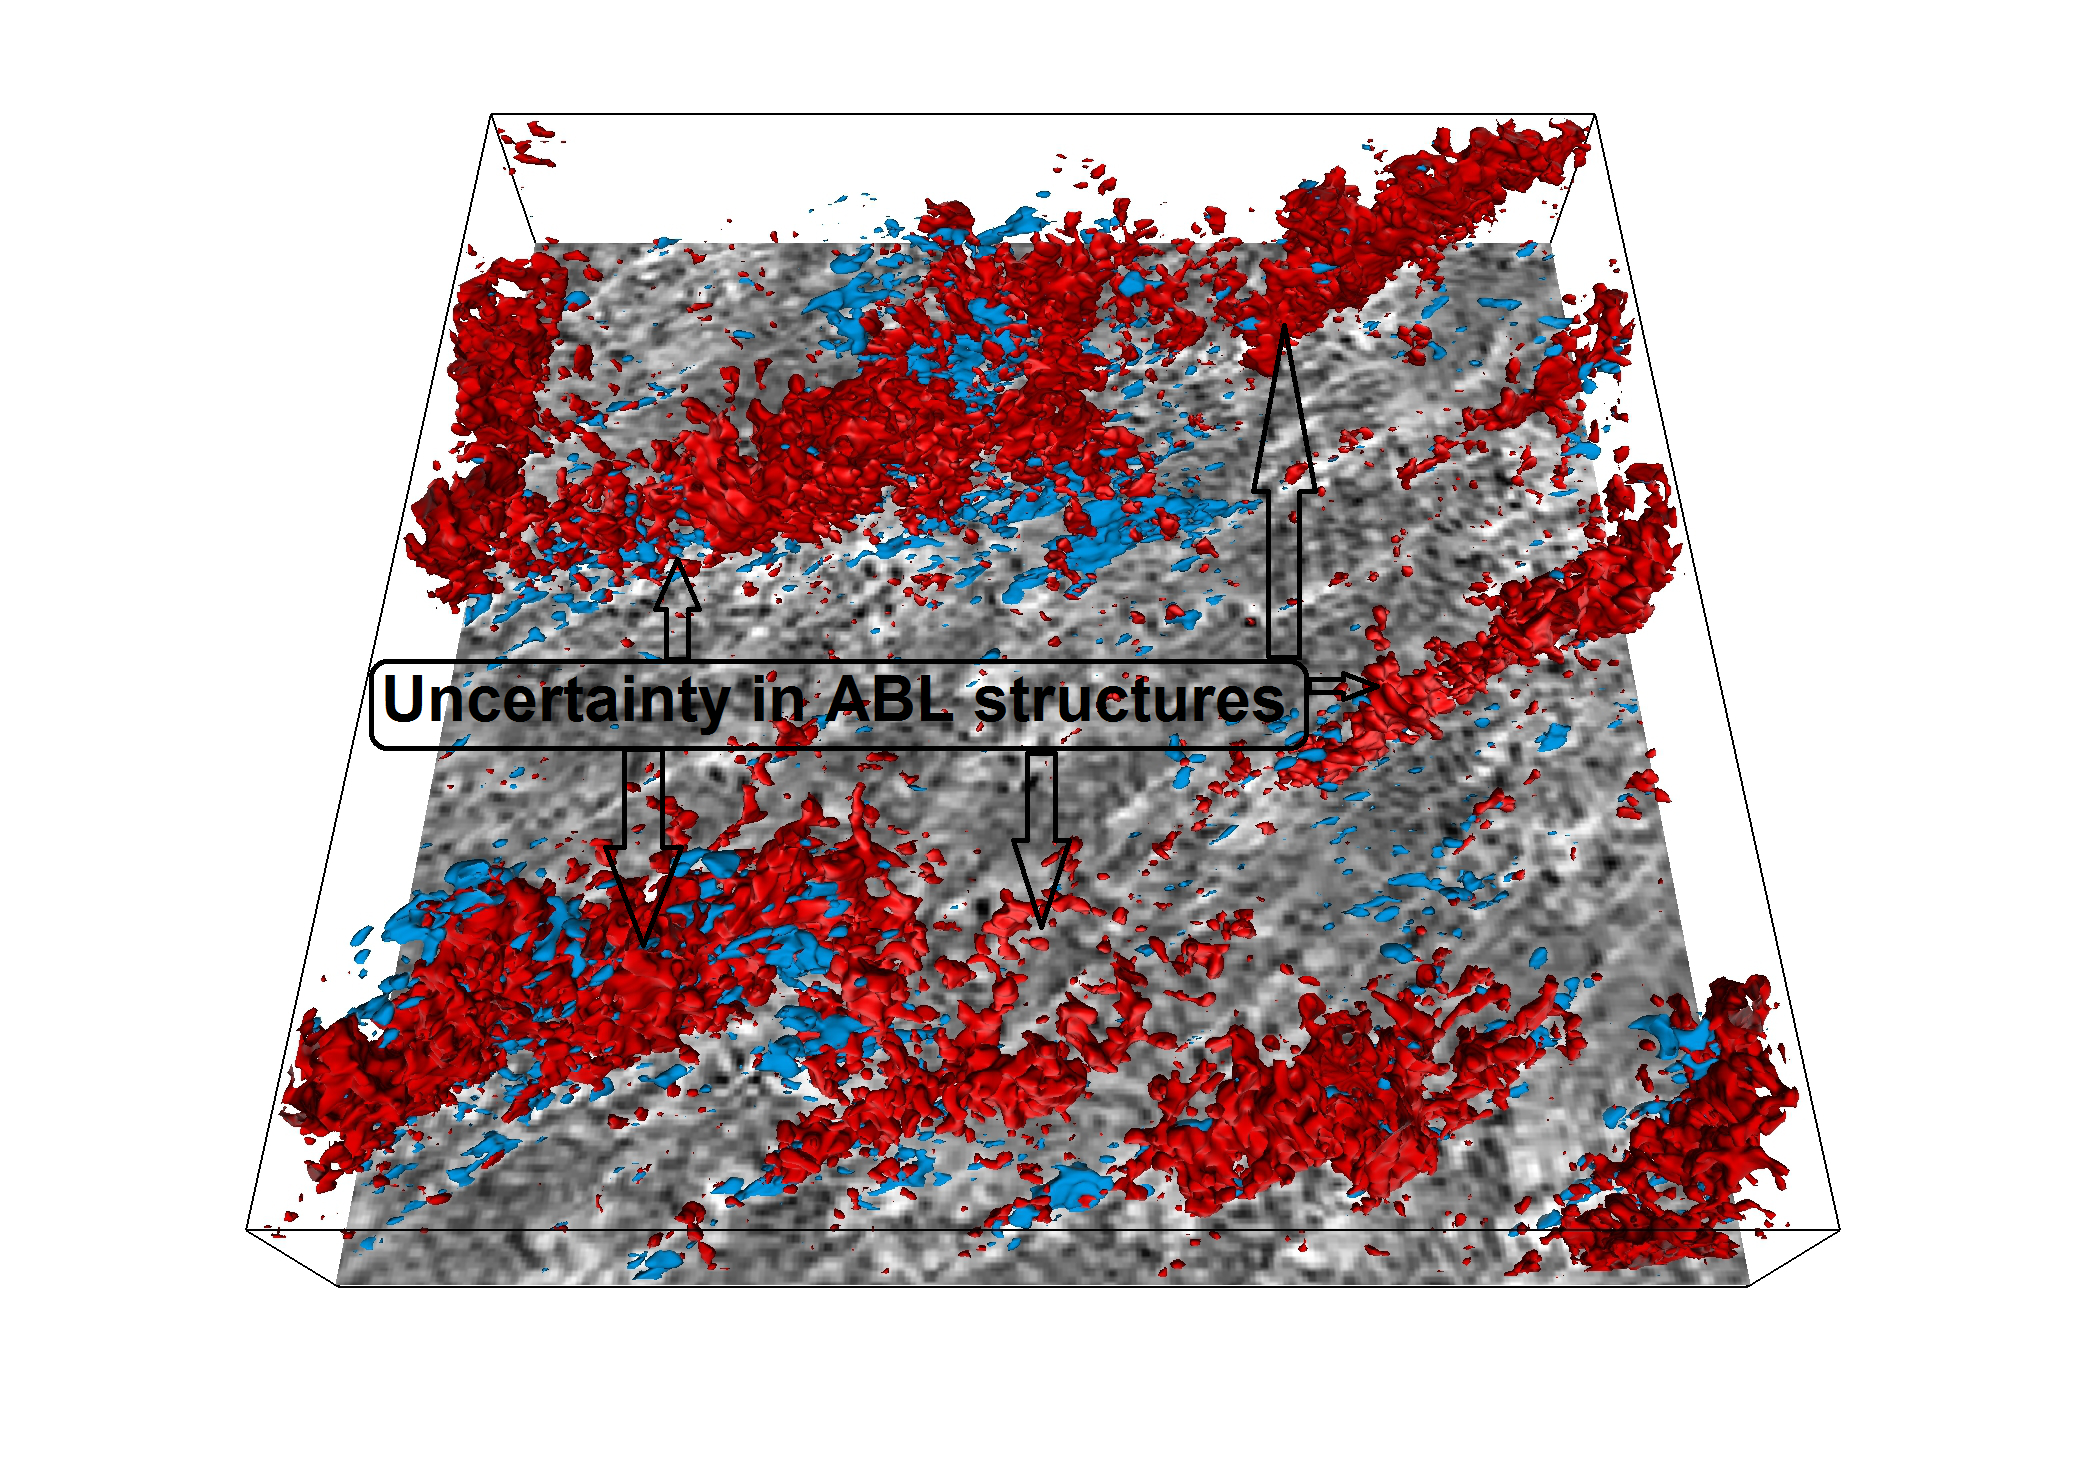
\includegraphics[scale=0.25]{UQ1.png}
 \caption{Iso-surface of instantaneous velocity fluctuations and aleatoric uncertainties.}
 \label{f:UQ1}
\end{figure}

\begin{figure}
 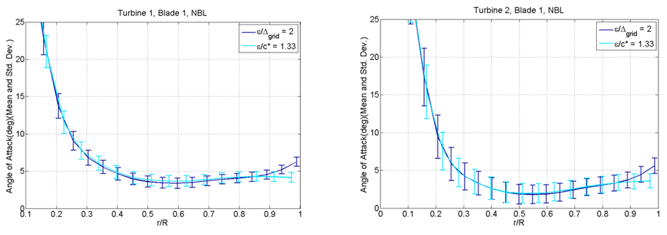
\includegraphics[scale=0.25]{ALM_discrepancy.png}
 \caption{Epistemic uncertainties in mean angle-of-attack (AOA). (a) Turbine 1 (NBL)    (b) Turbine 2 (NBL).}
 \label{f:ALM_discrepancy}
\end{figure}

\begin{figure}
 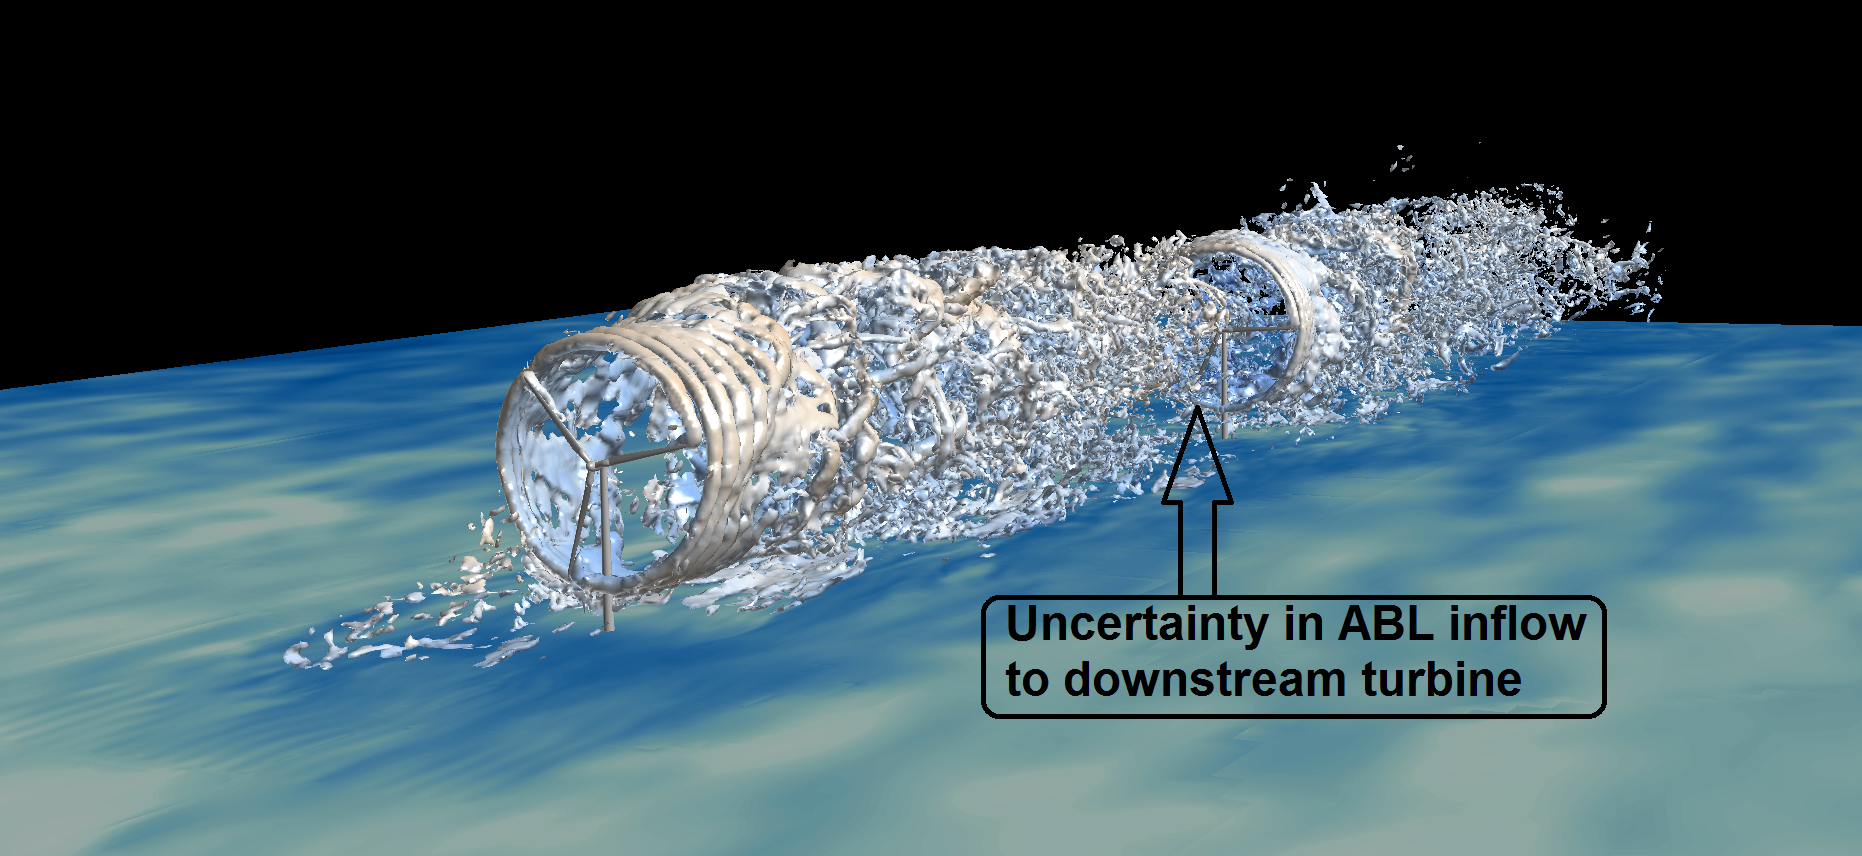
\includegraphics[scale=0.25]{UQ3.png}
 \caption{Uncertainties in the wake and inflow (aleatoric) to the downstream turbine.}
 \label{f:UQ3}
\end{figure}

From the above discussion of a turbine-turbine interaction problem, we can summarize the uncertainties identified so far:

Upstream turbine: 
\begin{itemize}
  \item Aleatoric uncertainty due to ABL (spatial and temporal variations).
  \item Epistemic uncertainty in the predicted blade loads and derived quantities such as power.
\end{itemize}

Downstream turbine: 
\begin{itemize}
  \item Aleatoric uncertainty due to ABL (spatial and temporal variations, which depend on ABL state), and the epistemic uncertainty in the blade loads (tip vortices) of the upstream turbine which have propagated in the wake.
  \item Epistemic uncertainty in the predicted blade loads and derived quantities such as power.
\end{itemize}

From this simple model of two turbines we can infer that, in a real wind farm with multiple turbines (could be around 50-100), the aleatoric uncertainty in inflow at a downstream turbine is the accumulation of epistemic uncertainty in the blade loads of all the upstream turbines. For a real wind farm, such as Lillgund,\cite{churchfield:aiaa2012} the accumulated uncertainties in the blade loads, power prediction, and wake profiles are anticipated to be much more pronounced than that discussed for the two-turbine example. Since these uncertainties are directly related to the structure and strength of the tip vortices, which determine the wake recovery process, the problem described needs a detailed investigation for a real wind farm.

In addition to the sources of uncertainties identified above, wake meandering can cause a severe wind shear in the horizontal and spanwise directions. Hence, the wake from a turbine and any epistemic uncertainty associated with it adds to the aleatoric uncertainty of each turbine affected by wake meandering. An idea of the propagation of uncertainties and wake meandering can be obtained from Figure \ref{f:UQ2}. It shows the flow-field of an array of five NREL 5-MW turbines, where the main row comprises three turbines and the sub-row comprises two. The iso-surface of vorticity magnitude 0.5 1/s is shown on the left and the iso-surface of velocity fluctuations (u’ = 2.5 m/s (blue), w’ = 2.0 m/s (red)) on the right. 

\begin{figure}
 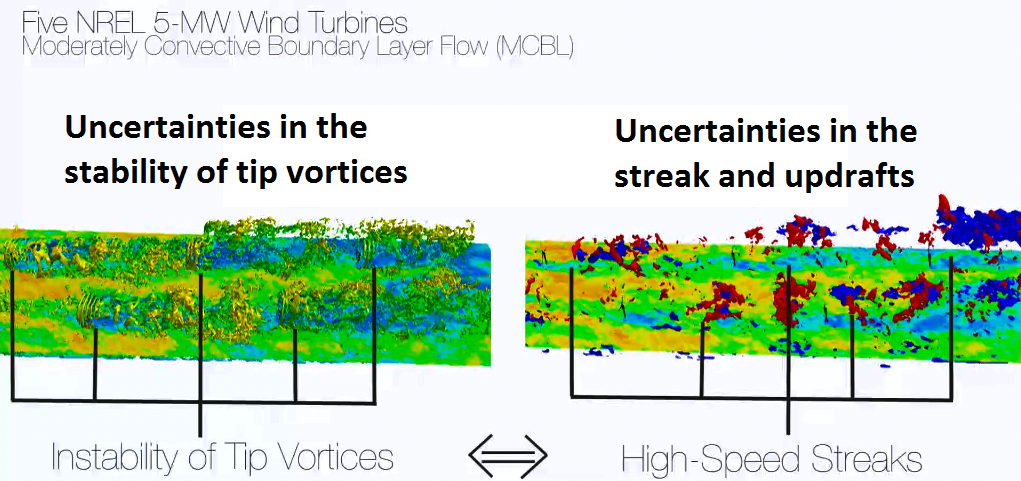
\includegraphics[scale=0.25]{UQ2.png}
 \caption{Uncertainties in tip vortices, streaks, and updrafts in a turbine array.}
 \label{f:UQ2}
\end{figure}

\section{Outlook to Full Paper}

The types of uncertainties in the inflow identified above and the analyses of simple two-turbine simulations would be extended to an array of several turbines in ascending order of complexity. The uncertainties associated with other models, such as higher-fidelity blade-resolved simulations, or some lower-fidelity models, will also be identified and quantified. A preliminary investigation involving fewer turbines than in an actual wind farm is proposed, where the issues of accruing uncertainty downstream and wake meandering are addressed. A 3 X 3 turbine array, i.e. 3 rows with 3 turbines each, would be a good candidate. A utility-scale turbine such as Envision EN136 4-MW turbine or NREL 5-MW turbine can be chosen for the trbine array. The detailed analysis would include statistics of blade loads for different turbines, integrated quantities such as power, thrust and bending moment, and wake parameters including velocity deficit, velocity fluctuation (and consequently Reynolds stresses signifying meandering and entrainment, and turbulent kinetic energy (TKE)). Studies on strength, propagation, and breakdown of tip vortices would also be included. 
Some of the uncertainty quantification algorithms to be used for the proposed analyses are latin hypercube sampling (LHS),\cite{iman:wiley2008}\textsuperscript{, }\cite{helton:re2003} stratified sampling, response surface method, and stochastic simplex collocation (SSC).\cite{witterveen:aiaa2010}\textsuperscript{-}\cite{witterveen:jcp2013} Another approach that can be used is to cast the physical process (ABL and turbine ALM) as a stochastic partial differential equation and its solution using deterministic methods such as perturbation expansion methods for random field, stochastic operator expansions, and polynomial chaos methods.\cite{najm:arfm2009} A successful accomplishment of the proposed work will meet some of the objectives of IEA Wakebench.

\begin{thebibliography}{9}% maximum number of references (for label width)

\bibitem{lackner:aiaa2007}
Lackner, M.A., Rogers, A.L., and Manwell, J.F., ``Uncertainty Analysis in Wind Resource Assessment and Wind Energy Production Estimation," AIAA 2007-1222.

\bibitem{lackner:asme2008}
Lackner, M.A., Rogers, A.L., and Manwell, J.F., ``Uncertainty Analysis in MCP-Based Wind Resource Assessment and Energy Production Estimation," ASME Journal of Solar Energy Engineering, 130(3), 031006 (Jul 01, 2008).

\bibitem{kwon:ae2010}
Kwon, S.D., ``Uncertainty analysis of wind energy potential assessment," Applied Energy, 87(3), pp 856-865.

\bibitem{jha:aiaa2014}
Jha, P. K., Churchfield, M. J., Moriarty, P. J., and Schmitz, S., ``The Effect of Various Actuator-Line   Modeling Approaches on Turbine-Turbine Interactions and Wake-Turbulence Statistics in Atmospheric Boundary-Layer Flow," AIAA 2014-0710.

\bibitem{jha:jsee2014}
Jha, P. K., Churchfield, M. J., Moriarty, P. J., and Schmitz, S., ``Guidelines for Volume Force  Distributions within Actuator Line Modeling of Wind Turbines on Large-Eddy Simulation-type Grids," ASME Journal of Solar Energy Engineering, 136(3), 0310014 (Jan 10, 2014).

\bibitem{churchfield:aiaa2012}
Churchfield, M. J., Lee, S., Moriarty, P. J., Martínez, L. A., Leonardi, S., Vijayakumar, G. and  Brasseur, J. G., ``A Large-Eddy Simulation of Wind-Plant Aerodynamics," AIAA 2012-0537.

\bibitem{iman:wiley2008}
Iman, R. L., ``Latin Hypercube Sampling," Encyclopedia of Quantitative Risk Analysis and Assessment, Wiley 2008

\bibitem{helton:re2003}
Helton, J.C. and Davis, F.J., ``Latin hypercube sampling and the propagation of uncertainty in analyses of complex systems," Reliability Engineering \& System Safety, 81(1), pp 23-69

\bibitem{witterveen:aiaa2010}
Witterveen, J.A.S. and Iaccarino, G., ``Simplex Elements Stochastic Collocation in Higher-Dimensional Probability Spaces." AIAA 2010-2924

\bibitem{witterveen:siam2012}
Witterveen, J.A.S. and Iaccarino, G., ``Simplex Stochastic Collocation with Random Sampling and Extrapolation for Nonhypercube Probability Spaces," SIAM J. Sci. Comput., 34(2), pp A814–A838.

\bibitem{witterveen:jcp2013}
Witterveen, J.A.S. and Iaccarino, G., ``Simplex stochastic collocation with ENO-type stencil selection for robust uncertainty quantification, Journal of Computational Physics, Volume 239, 15 April 2013, pp 1-21.

\bibitem{najm:arfm2009}
Najm, H. N., ``Uncertainty Quantification and Polynomial Chaos Techniques in Computational Fluid Dynamics," Annual Review of Fluid Mechanics
Vol. 41, pp 35-52. 


\end{thebibliography}

\end{document}

% - Release $Name:  $ -
